\section{Gli Alberi di Decisione (AI)}

% ------------------------------------------------------------
\subsection{Concetti Fondamentali e Rappresentazione}
% ------------------------------------------------------------

Nell'ambito dei sistemi di classificazione, gli alberi di
decisione rappresentano un metodo intuitivo per classificare
un pattern attraverso una sequenza di domande. La logica
sottostante prevede che la domanda successiva dipenda
strettamente dalla risposta fornita al quesito corrente,
creando così un percorso ramificato. Questo strumento risulta
particolarmente utile quando si trattano dati non metrici
(\textit{nominal data}). Le risposte ammissibili possono
essere binarie (Sì/No, Vero/Falso) oppure appartenere a un
insieme definito di valori di proprietà. Grazie alla loro
capacità di gestire valori discreti, gli alberi di decisione
sono una scelta comune per gli scenari di rete.

Per quanto riguarda la rappresentazione formale, gli alberi
di decisione classificano le istanze ordinandole lungo la
struttura dell'albero, partendo dal
\textit{Root Node} fino a raggiungere un
\textit{Leaf Node}. In questa
architettura, ogni nodo specifica un test su un determinato
attributo dell'istanza in esame. Ogni ramo discendente da
un nodo corrisponde a uno dei possibili valori per
l'attributo testato. Il processo termina quando si raggiunge
una foglia, la quale fornisce la classificazione finale.

% ............................................................
\paragraph{Esempio di Training Set e Struttura}
% ............................................................

Considerato un
training set composto da eventi di rete (E1 a E13)
caratterizzati da attributi quali:

\begin{itemize}
    \item \textbf{Protocol}: TCP, ICMP, UDP
    \item \textbf{Data Size}: Large, Med, Low
    \item \textbf{Dest Port}: Well-Known, Other
    \item \textbf{Dest IP}: Internal, External
\end{itemize}

L'obiettivo è classificare se tali eventi rappresentino
traffico di gestione (\textit{Mgmt Traffic}: Yes/No).
Ad esempio, l'evento E1 (TCP, Large, Well-Known, Internal)
è classificato come ``No'', mentre l'evento E3 (ICMP)
è classificato come ``Yes''.

Graficamente, un albero di decisione parte da un attributo
radice, come ``Protocol''. Da questo nodo si diramano tre
possibilità: TCP, ICMP e UDP. Se il protocollo è ICMP,
l'albero conduce direttamente a ``Yes''. Se è TCP o UDP,
il percorso prosegue verso nodi interni che testano altri
attributi (Dest Port, Dest IP). In sintesi, ogni nodo
interno testa un attributo $X_i$, mentre ogni ramo seleziona
uno specifico valore per $X_i$.

\begin{figure}[H]
    \centering
    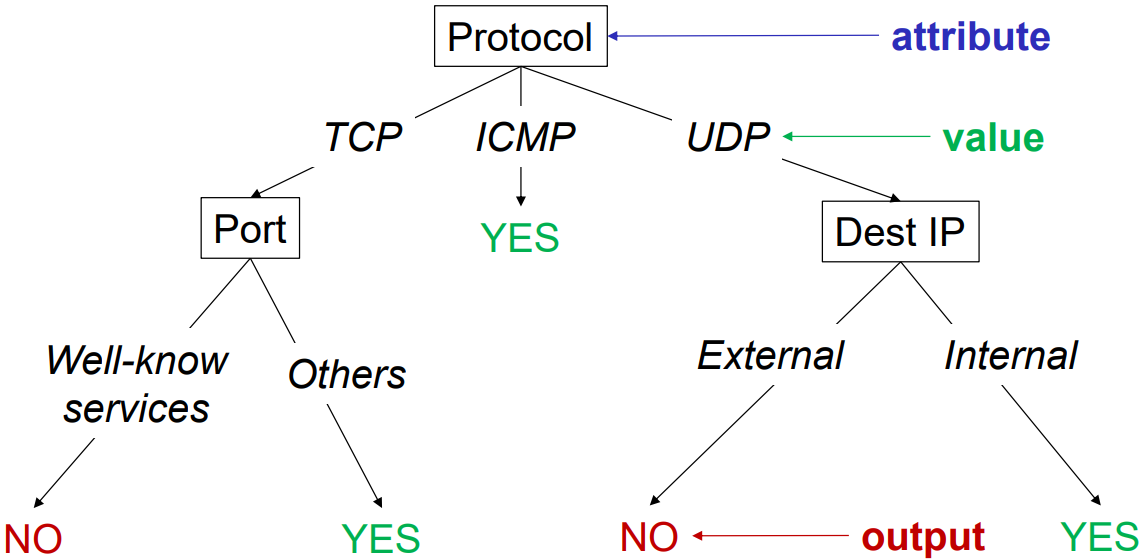
\includegraphics[width=0.5\textwidth]{img/decisionTree.png}
\end{figure}

% ------------------------------------------------------------
\subsection{Caratteristiche del Modello e Algoritmo
di Costruzione}
% ------------------------------------------------------------

Il modello si basa su una \textbf{descrizione
attributo-valore}: ogni oggetto deve essere esprimibile in
termini di una collezione fissa di proprietà o attributi.
Se si dispone di attributi continui, è necessario
discretizzarli oppure tale discretizzazione deve essere
prevista all'interno dell'algoritmo stesso.

Un altro requisito essenziale è l'esistenza di
\textbf{classi predefinite} (\textit{target attribute
value}). Le categorie devono essere stabilite a priori,
configurando il problema nell'ambito dell'apprendimento
supervisionato. Inoltre le classi devono essere discrete:
un caso appartiene o non appartiene a una particolare
classe. È necessario che vi siano più casi (esempi)
rispetto al numero delle classi disponibili.

% ............................................................
\subsubsection{Pseudo-Codice e Dati Sufficienti}
% ............................................................

Per costruire un albero efficace, è imperativo disporre di
\textbf{dati sufficienti}. Generalmente sono necessarie
centinaia o migliaia di casi di addestramento per garantire
una buona generalizzazione.

Il processo algoritmico segue una modalità ben definita:

\begin{enumerate}
    \item \textbf{Inizializzazione}: si testano tutti gli
        attributi per selezionare quello che performa
        meglio come radice (\textit{best root}).
    \item \textbf{Main Loop}: si assegna $A$ come il
        miglior attributo decisionale per il nodo corrente.
        Per ogni valore possibile $v_i \in A$, si crea un
        nodo discendente. Gli esempi di addestramento
        vengono ordinati verso il nodo figlio appropriato.
    \item Il processo continua iterativamente finché tutti
        gli esempi non sono stati classificati.
\end{enumerate}

Si tratta in sostanza di una ricerca \textit{greedy} volta
a trovare un albero decisionale accettabile.

% ------------------------------------------------------------
\subsection{Selezione degli Attributi: Impurità
ed Entropia}
% ------------------------------------------------------------

Una questione critica nella costruzione dell'albero riguarda
la selezione degli attributi: quale attributo deve essere
scelto successivamente, $A_1$ o $A_2$? L'obiettivo è
cercare un attributo che renda i dati che raggiungono
i nodi discendenti immediati il più \textit{puri}
possibile.

Per operare questa scelta, è più conveniente definire il
concetto opposto: l'\textbf{impurità} (\textit{impurity})
di un nodo. Un gruppo \textit{molto impuro} contiene una
mescolanza eterogenea di classi, mentre un gruppo con
\textit{impurità minima} contiene prevalentemente elementi
di una sola classe.

\begin{figure}[H]
    \centering
    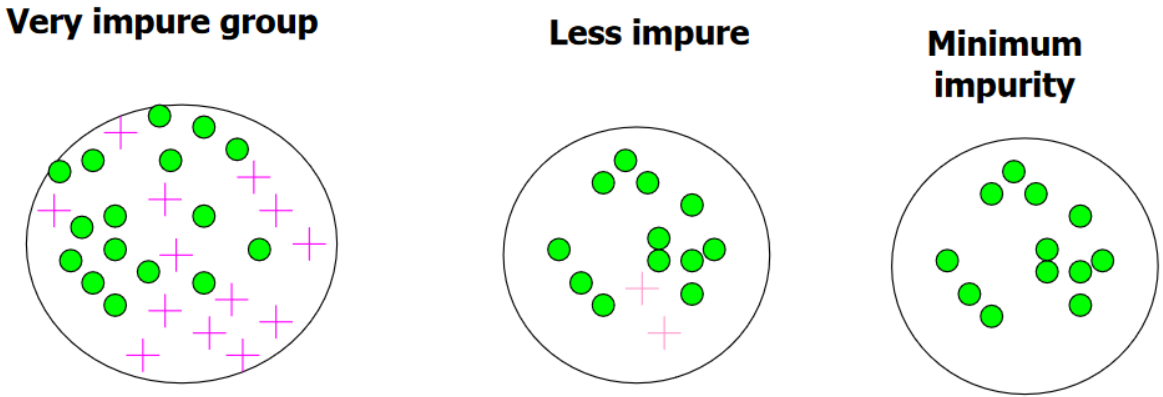
\includegraphics[width=0.6\textwidth]{img/impurity.png}
\end{figure}

Definiamo $i(N)$ come l'impurità di un nodo $N$:
\begin{itemize}
    \item $i(N) = 0$ se tutti i pattern appartengono alla
        stessa categoria.
    \item $i(N)$ grande se tutte le categorie sono
        equamente rappresentate.
\end{itemize}

La misura più popolare è l'\textbf{entropia}
(\textit{Entropy Impurity}):

\begin{equation}
    i(N) = -\sum_{j=1}^{n} P(w_j) \log_2 P(w_j)
\end{equation}

dove $P(w_j)$ è la frazione di pattern al nodo $N$ che
appartengono alla categoria $w_j$.

L'entropia $H(X)$ di una variabile casuale discreta $X$,
con due sole classi $w_+$ e $w_-$, è:

\begin{equation}
    H(X) = -P(w_+)\log_2 P(w_+) - P(w_-)\log_2 P(w_-)
\end{equation}

Se la probabilità di una classe è 0 e dell'altra è 1
(massima purezza), l'entropia $H(X) = 0$. Il picco massimo
(valore 1) si raggiunge quando le probabilità sono uguali
(0.5), indicando la massima impurità.

% ............................................................
\subsubsection{Guadagno di Informazione
(Information Gain)}
% ............................................................

L'entropia deriva dalla teoria dell'informazione: maggiore
è l'entropia, maggiore è il contenuto informativo
intrinseco, ovvero l'incertezza da risolvere.

Per costruire l'albero, si sceglie l'attributo che riduce
maggiormente l'impurità del nodo. Questa metrica è chiamata
\textbf{guadagno di informazione} (\textit{Information
Gain}), che misura la riduzione attesa di entropia dovuta
all'ordinamento basato sull'attributo $A$:

\begin{equation}
    Gain(S, A) = i(S) -
    \sum_{v \in Values(A)} \frac{|S_v|}{|S|} \, i(S_v)
\end{equation}

dove $S$ è l'insieme originale, $S_v$ è il sottoinsieme
di $S$ per cui l'attributo $A$ ha valore $v$, e $i(S_v)$
è l'entropia di quel sottoinsieme. In pratica, si sottrae
all'entropia originale la somma ponderata delle entropie
dei sottoinsiemi creati dalla divisione.

\begin{figure}[H]
    \centering
    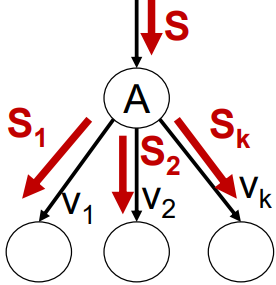
\includegraphics[width=0.3\textwidth]{img/infoGain.png}
\end{figure}

% ------------------------------------------------------------
\subsection{Esempio Pratico di Calcolo}
% ------------------------------------------------------------

\begin{figure}[H]
    \centering
    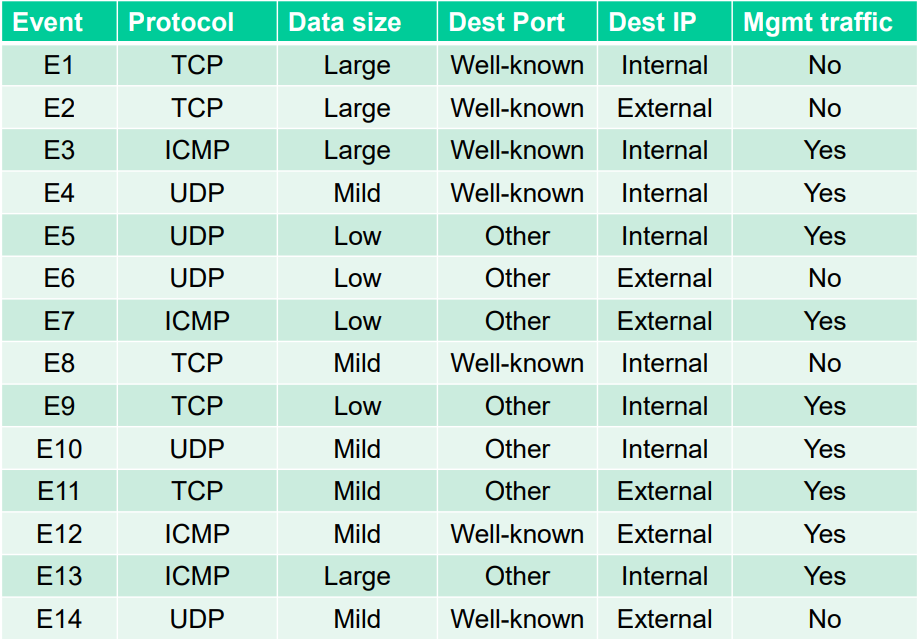
\includegraphics[width=0.6\textwidth]{img/training1.png}
\end{figure}

Il set completo include 14 eventi (E1--E14). Rappresentiamo
con la notazione $E[X+,\, Y-]$ il fatto che vi siano $X$
elementi positivi (Yes) e $Y$ negativi (No). Su 14 esempi
totali, 9 sono ``Sì'' e 5 sono ``No'', quindi:

\begin{equation}
    i(S) = E[9+,\, 5-] =
    -\!\left(\frac{9}{14}\log_2\frac{9}{14}\right)
    -\!\left(\frac{5}{14}\log_2\frac{5}{14}\right)
    = 0.94
\end{equation}

% ............................................................
\subsubsection{Calcolo del Guadagno dell'Attributo}
% ............................................................

Il passo successivo consiste nel calcolare $Gain(S, A)$
per ciascun attributo $A \in \{$Protocol, Data Size,
Dest Port, Dest IP$\}$.

\paragraph{Attributo Protocol.}
Divide i dati in tre sottoinsiemi:
TCP $(2+, 3-)$, ICMP $(4+, 0-)$, UDP $(3+, 2-)$.

\begin{equation}
    \begin{aligned}
        \mathrm{Gain}(S,\,\text{Protocol})
        &= i(S) - \left[\frac{5}{14}\,i(\text{Protocol}=\text{TCP})
        + \frac{4}{14}\,i(\text{Protocol}=\text{ICMP})
        + \frac{5}{14}\,i(\text{Protocol}=\text{UDP})\right] \\
        &= E([9+,5-]) - \left[\frac{5}{14}E([2+,3-])
        + \frac{4}{14}E([4+,0-])
        + \frac{5}{14}E([3+,2-])\right] \\
        &= 0.94 - \left[\frac{5}{14}\cdot 0.971
        + \frac{4}{14}\cdot 0.0
        + \frac{5}{14}\cdot 0.971\right] = 0.246
    \end{aligned}
\end{equation}

\paragraph{Attributo Data Size.}
Divide i dati in Large, Med, Low:

\begin{equation}
    0.94 -
    \left[\frac{4}{14}\cdot 1
    + \frac{6}{14}\cdot 0.918
    + \frac{4}{14}\cdot 0.811\right]
    = 0.029
\end{equation}

\paragraph{Attributo Dest Port.}
$Gain = 0.1515$, calcolato separando
i casi ``Well-Known'' da quelli ``Other''.

\paragraph{Attributo Dest IP.}
$Gain = 0.048$.

Confrontando i risultati $(0.246,\ 0.029,\ 0.1515,\ 0.048)$,
si conclude che \textbf{Protocol è il vincitore} in quanto
offre il maggiore guadagno di informazione. L'albero inizia
quindi con il nodo radice ``Protocol''. I rami si dividono
in:

\begin{itemize}
    \item \textbf{TCP}: eventi $\{E1, E2, E8, E9, E11\}$
        con entropia $0.971$.
    \item \textbf{ICMP}: eventi $\{E3, E7, E12, E13\}$
        con entropia $0.0$ (tutti positivi
        $\rightarrow$ foglia ``Yes'').
    \item \textbf{UDP}: eventi $\{E4, E5, E6, E10, E14\}$
        con entropia $0.971$.
\end{itemize}

% ............................................................
\subsubsection{Sviluppo Ricorsivo dei Rami}
% ............................................................

Avendo stabilito la radice, si trovano ricorsivamente i
nodi sotto i rami TCP e UDP (il ramo ICMP è già risolto).

\paragraph{Ramo Protocol = UDP.}
Si ricalcola il guadagno per gli attributi rimanenti:
\begin{align*}
    Gain(\text{Protocol=UDP},\ \text{Dest Port})
        &= 0.02 \\
    Gain(\text{Protocol=UDP},\ \text{Dest IP})
        &= 0.971 \\
    Gain(\text{Protocol=UDP},\ \text{Data Size})
        &= 0.02 
\end{align*}
Il valore molto alto per Dest IP suggerisce che questo
sarà il prossimo nodo discriminante per il ramo UDP.

\paragraph{Ramo Protocol = TCP.}
Si determina quale attributo selezionare per il
sottoinsieme $S_{TCP} = \{E1, E2, E8, E9, E11\}$:
\begin{align*}
    Gain(\text{TCP},\ \text{Dest Port}) &= 0.97 \\
    Gain(\text{TCP},\ \text{Data Size}) &= 0.57 \\
    Gain(\text{TCP},\ \text{Dest IP}) &= 0.019
\end{align*}
Dest Port risulta il nodo discriminante per il ramo TCP.

% ............................................................
\subsubsection{Terminazione e Rasoio di Occam}
% ............................................................

Il processo ricorsivo continua per ogni nuovo nodo finché
non viene soddisfatta una delle due condizioni seguenti:

\begin{itemize}
    \item Ogni attributo è già stato incluso lungo questo
        percorso attraverso l'albero.
    \item Gli esempi di addestramento arrivati a questo
        nodo foglia hanno tutti lo stesso valore
        dell'attributo target (entropia = 0).
\end{itemize}

Nel nostro esempio si verifica il secondo caso: l'attributo
``Data Size'' non viene incluso nell'albero risultante,
in quanto non necessario per completare la classificazione.

L'albero risultante ha la seguente struttura:
\begin{itemize}
    \item Radice: \textbf{Protocol}
    \item Ramo ICMP $\rightarrow$ \textbf{Yes}
    \item Ramo TCP $\rightarrow$ test su
        \textbf{Dest Port}:
        Well-Known $\rightarrow$ No,
        Other $\rightarrow$ Yes
    \item Ramo UDP $\rightarrow$ test su
        \textbf{Dest IP}:
        External $\rightarrow$ No,
        Internal $\rightarrow$ Yes
\end{itemize}

L'algoritmo descritto, noto come \textbf{ID3}, esegue una
ricerca euristica attraverso lo spazio degli alberi
decisionali, partendo dal più semplice al più complesso,
guidato dal guadagno di informazione. Si ferma al più
piccolo albero accettabile. Questo metodo si rifà al
\textbf{Rasoio di Occam}: si deve preferire l'ipotesi
più semplice che si adatta ai dati.

% ------------------------------------------------------------
\subsection{Overfitting e Gestione del Rumore}
% ------------------------------------------------------------

Esistono diverse ragioni per preferire la semplicità.
In primo luogo, il numero di ipotesi semplici che possono
``adattarsi accidentalmente'' ai dati è piccolo; di
conseguenza è probabile che un'ipotesi semplice scopra
una conoscenza interessante sui dati. In secondo luogo,
gli alberi più semplici non partizionano lo spazio delle
caratteristiche in troppe piccole ``scatole'', permettendo
di generalizzare meglio. Al contrario, gli alberi complessi
rischiano di diventare una scatola separata per ogni
singolo campione di addestramento, portando al fenomeno
dell'\textbf{overfitting} (sovraddattamento).

% ............................................................
\subsubsection{Overfitting in Decision Tree}
% ............................................................

Consideriamo l'effetto dell'aggiunta di un esempio rumoroso
(\textit{noisy example}) al dataset. Immaginiamo un nuovo
evento E14 con le seguenti caratteristiche: TCP, Data Size
Large, Dest Port Other, Dest IP External, Mgmt Traffic = No.

La domanda è: come influisce questo dato sull'albero
decisionale costruito? La presenza di rumore nei dati,
o l'incoerenza di un piccolo numero di esempi, può alterare
significativamente la struttura se non gestita correttamente.

% ............................................................
\subsubsection{Tecniche per Evitare l'Overfitting}
% ............................................................

Come possiamo evitare il sovraddattamento? Un metodo
efficace è la \textbf{potatura dell'albero}
(\textit{pruning}), ovvero renderlo più piccolo rimuovendo
i nodi che non risultano utili. Esistono due approcci
principali:

\begin{itemize}
    \item \textbf{Pre-pruning}: smettere di far crescere
        l'albero in anticipo, prima che classifichi
        perfettamente i dati di addestramento.
    \item \textbf{Post-pruning}: far crescere l'albero
        completo e successivamente potarlo.
\end{itemize}

%-------------------------------------------------------
%-------------------------------------------------------
%-------------------------------------------------------
%-------------------------------------------------------

% ------------------------------------------------------------
\subsection{Pre-Pruning: Criteri e Risultati}
% ------------------------------------------------------------

Nell'ambito dell'ottimizzazione degli alberi di decisione,
il \textbf{pre-pruning} (potatura preventiva) consiste
nell'interrompere la crescita dell'albero prima che raggiunga
la sua massima espansione possibile. Esistono diversi criteri
per determinare quando fermare questo processo:

\begin{itemize}
    \item \textbf{Maximum depth}: profondità massima
        dell'albero, che ne limita l'estensione verticale.
    \item \textbf{Minimum samples for split}: numero
        minimo di campioni in un nodo per giustificare
        una nuova ramificazione.
    \item \textbf{Num samples per leaf} ($n_L$): numero
        minimo di istanze che ogni nodo foglia deve
        contenere.
    \item \textbf{Maximum number of leaf nodes}: limite
        al numero totale di nodi foglia nell'albero.
    \item \textbf{Minimum impurity decrease}: le
        divisioni sono consentite solo se riducono
        l'impurezza di una quantità specificata.
\end{itemize}

% ............................................................
\subsubsection{Minimum Samples per Leaf: Esempio}
% ............................................................

Per comprendere meglio il criterio del numero minimo di
campioni per foglia, si consideri un esempio con il
parametro \texttt{MinNumObjects} impostato a 30. In una
situazione in cui un nodo $E_4$ contiene 43 oggetti
(34 negativi e 9 positivi) e una divisione proposta
separerebbe questi in un gruppo di 34 e uno di 9, la
regola viene violata: il gruppo con 9 oggetti è inferiore
alla soglia di 30. Di conseguenza, la divisione viene
annullata e i nodi vengono accorpati, terminando la
crescita in quel punto.

\begin{figure}[H]
\centering
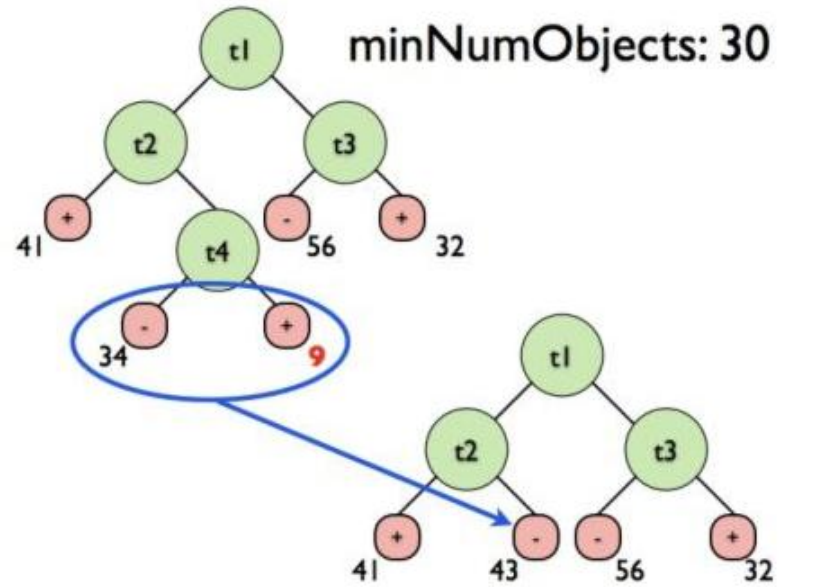
\includegraphics[width=0.6\textwidth]{img/minLeaf.png}
\end{figure}

% ............................................................
\subsubsection{Quando Usare il Pre-Pruning?}
% ............................................................

L'utilizzo del pre-pruning è particolarmente indicato
nei seguenti scenari:

\begin{itemize}
    \item \textbf{Dataset di grandi dimensioni}: arrestare
        precocemente la crescita dell'albero evita di
        catturare il rumore nei dati.
    \item \textbf{Rischio di overfitting elevato}: la
        tecnica riduce la complessità del modello prima
        ancora che si manifesti il problema.
    \item \textbf{Riduzione dei tempi di addestramento}:
        alberi più piccoli sono più veloci da costruire
        e più facili da interpretare.
\end{itemize}

Tuttavia, esiste un rischio intrinseco: il potenziale
\textbf{underfitting}. Se i criteri di arresto vengono
impostati in modo troppo rigoroso, l'albero potrebbe non
catturare pattern importanti presenti nei dati,
compromettendo la capacità predittiva del modello.

% ------------------------------------------------------------
\subsection{Post-Pruning: Algoritmo e Cost-Complexity}
% ------------------------------------------------------------

Per superare i limiti del pre-pruning, si ricorre al
\textbf{post-pruning}. Questo algoritmo utilizza una
ricerca \textit{greedy hill-climbing} per potare l'albero
dopo che è stato completamente costruito. Il funzionamento
procede in modo iterativo:

\begin{enumerate}
    \item Per ogni nodo interno (non foglia) si ipotizza
        di rimuovere il sotto-albero che ha origine in $n$.
    \item Tale sotto-albero viene sostituito con un nodo
        foglia, a cui viene assegnata l'etichetta di classe
        in base alla maggioranza degli esempi di
        addestramento che ricadono in quel sotto-albero.
    \item Si misura la performance del nuovo albero
        usando un \textbf{validation set} separato e
        si memorizza l'albero con le prestazioni migliori.
    \item Il processo si ripete finché la rimozione di
        qualsiasi nodo interno non porta più ad alcun
        miglioramento.
\end{enumerate}

Se un albero potato presenta le stesse prestazioni
dell'albero corrente, si preferisce quello potato per
via della sua maggiore semplicità.

% ............................................................
\subsubsection{Criteri di Selezione per il Post-Pruning}
% ............................................................

Esistono diversi criteri per selezionare quali rami tagliare:

\begin{itemize}
    \item \textbf{Cost-Complexity Pruning (CCP)}: assegna
        un costo a ciascun sotto-albero basandosi su
        accuratezza e complessità, selezionando quello
        con il costo più basso.
    \item \textbf{Reduced Error Pruning}: rimuove i rami
        che non incrementano significativamente
        l'accuratezza complessiva.
    \item \textbf{Minimum Impurity Decrease}: pota i nodi
        se la riduzione di impurezza (Gini o entropia)
        è al di sotto di una certa soglia.
    \item \textbf{Minimum Leaf Size}: rimuove i nodi
        foglia che contengono meno campioni di un
        numero stabilito.
\end{itemize}

% ............................................................
\subsubsection{Dettagli del Cost-Complexity Pruning}
% ............................................................

Il metodo CCP (\textit{Cost-Complexity Pruning}) mira a
scambiare complessità per accuratezza nell'albero $T$.
L'obiettivo è minimizzare la seguente funzione di costo:

\begin{equation}
    \min Cost = \min \{ |T| + \alpha \, R(T) \}
\end{equation}

dove:
\begin{itemize}
    \item $|T|$ è la dimensione dell'albero, ovvero il
        numero di foglie ($N_{\text{leaves}}$).
    \item $R(T)$ indica gli errori di classificazione alle
        foglie, e si può scrivere come:
        \begin{equation}
            R(T) = \frac{1}{N}\sum_{L \in \text{leaves}} I(L)\, n_L
        \end{equation}
        calcolato sommando su tutte le
    foglie L il prodotto dell'impurezza I(L) per la proporzione di campioni 
    in quella foglia $n_L$.
    \item $\alpha$ è il parametro di complessità, che
        determina il fattore di influenza tra complessità
        e performance.
    \item $n_L$ è il numero di campioni sulla foglia $L$.
    \item $P_L$ è la frazione di etichette rilevante
        sulla foglia $L$.
\end{itemize}

A parità di costo (errore di classificazione), si
seleziona il sotto-albero con più nodi, ovvero quello
con complessità maggiore, per favorire il modello più
semplice tra quelli con pari prestazioni.

% ............................................................
\subsubsection{Confronto Pre-Pruning e Post-Pruning}
% ............................................................

Le due tecniche presentano differenze sostanziali che
è utile mettere in luce:

\begin{table}[h!]
\centering
\begin{tabular}{lll}
\toprule
\textbf{Aspetto} &
\textbf{Pre-Pruning} &
\textbf{Post-Pruning} \\
\midrule
Crescita albero &
Arrestata in anticipo &
Completa, poi tagliata \\
Rischio principale &
Underfitting &
Costo computazionale \\
Velocità &
Più veloce &
Più lento \\
Dataset richiesto &
Solo training set &
Training + validation \\
Controllo &
Tramite iper-parametri &
Basato su validazione \\
\bottomrule
\end{tabular}
\end{table}

Il post-pruning offre una migliore generalizzazione
poiché il modello considera tutti i pattern possibili
prima di scartare quelli irrilevanti. Si raccomanda
quando il dataset è piccolo e l'overfitting è evidente,
oppure per affinare la complessità dell'albero. Il
pre-pruning è invece preferibile con dataset di grandi
dimensioni, dove il costo computazionale del costruire
l'albero completo sarebbe proibitivo.

% ------------------------------------------------------------
\subsection{Conversione in Regole e Valutazione Finale}
% ------------------------------------------------------------

Un'alternativa alla procedura standard di potatura è la
\textbf{conversione in regole} (\textit{Rule Post-Pruning}).
Questo processo prevede i seguenti passi:

\begin{enumerate}
    \item Far crescere l'albero finché i dati di
        addestramento non sono adattati al meglio
        possibile.
    \item Convertire l'albero appreso in un set
        equivalente di regole, creando una regola per
        ciascun percorso dalla radice a una foglia.
    \item Eliminare gli antecedenti non necessari:
        per le regole con due o più condizioni, si
        rimuovono quelle che non influenzano la
        conclusione raggiunta.
    \item Riordinare le regole in una sequenza ordinata
        per l'uso finale.
\end{enumerate}

Ad esempio, dall'albero con radice ``Protocol'' costruito
nel capitolo precedente si ottengono le regole:

\begin{itemize}
    \item \texttt{IF} (Protocol = TCP)
        \texttt{AND} (Dest Port = `Well-Known')
        \texttt{THEN} Mgmt Traffic = `No'
    \item \texttt{IF} (Protocol = TCP)
        \texttt{AND} (Dest Port = `Other')
        \texttt{THEN} Mgmt Traffic = `Yes'
    \item \texttt{IF} (Protocol = ICMP)
        \texttt{THEN} Mgmt Traffic = `Yes'
    \item \texttt{IF} (Protocol = UDP)
        \texttt{AND} (Dest IP = `External')
        \texttt{THEN} Mgmt Traffic = `No'
    \item \texttt{IF} (Protocol = UDP)
        \texttt{AND} (Dest IP = `Internal')
        \texttt{THEN} Mgmt Traffic = `Yes'
\end{itemize}

% ............................................................
\subsubsection{Punti di Forza e Debolezze degli Alberi
di Decisione}
% ............................................................

Gli alberi di decisione possiedono specifici punti di
forza (\textit{Strengths}):

\begin{itemize}
    \item Generano \textbf{regole comprensibili},
        rendendo il modello trasparente e interpretabile.
    \item Eseguono la classificazione senza richiedere
        una computazione eccessiva in fase di test.
    \item Gestiscono sia \textbf{variabili continue}
        che \textbf{categoriche}.
    \item Forniscono una chiara indicazione di quali
        feature siano più importanti per la predizione.
\end{itemize}

Esistono tuttavia debolezze intrinseche
(\textit{Weaknesses}):

\begin{itemize}
    \item Meno adatti per compiti di \textbf{regressione},
        dove l'obiettivo è predire un valore continuo.
    \item Inclini a errori in problemi con \textbf{molte
        classi} e pochi esempi di addestramento.
    \item \textbf{Costo computazionale} elevato in
        addestramento: ad ogni nodo ogni attributo
        candidato deve essere valutato; gli algoritmi
        di potatura possono risultare ulteriormente
        onerosi.
    \item Non trattano bene le \textbf{regioni non
        rettangolari}: la maggior parte degli algoritmi
        esamina un singolo attributo alla volta,
        producendo scatole di classificazione ortogonali
        agli assi che potrebbero non corrispondere
        alla distribuzione reale dei dati.
\end{itemize}

% ------------------------------------------------------------
\subsection{Trade-off Bias-Varianza}
% ------------------------------------------------------------

Per comprendere a fondo le prestazioni dei modelli di
machine learning, è necessario introdurre il compromesso
tra \textbf{bias} (distorsione) e \textbf{varianza}.
L'errore di bias è l'errore dovuto alle assunzioni
semplificative fatte dal modello per rendere la funzione
target più facile da apprendere. Modelli come KNN hanno
basso bias, mentre la regressione logistica e lineare
hanno alto bias.

L'errore di varianza rappresenta quanto la stima della
funzione target cambierebbe se venissero forniti dati di
addestramento diversi. Il KNN ha alta varianza, mentre
la regressione lineare e logistica ne hanno poca. Il
trade-off consiste nell'impostare gli iper-parametri
dell'algoritmo per bilanciare questi due aspetti. Nel
KNN, ad esempio, aumentare $K$ riduce la varianza ma
aumenta il bias.

\begin{figure}[H]
\centering
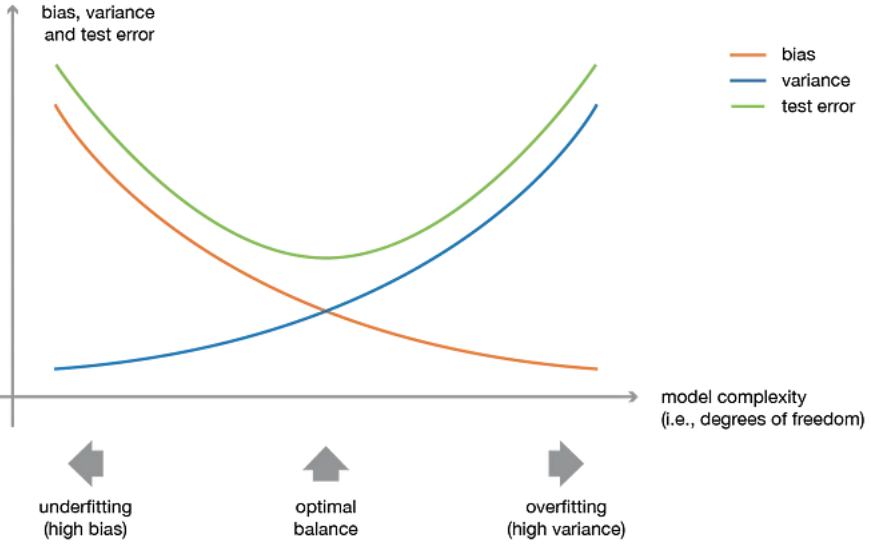
\includegraphics[width=0.6\textwidth]{img/biasVariance.png}
\end{figure}

% ............................................................
\subsubsection{Bias-Varianza negli Alberi di Decisione}
% ............................................................

Applicando questi concetti agli alberi di decisione,
possiamo affermare che i DT hanno \textbf{basso bias}
poiché non fanno assunzioni sulla funzione di target.
D'altra parte, i DT presentano \textbf{alta varianza}:
l'algoritmo divide i dati ripetutamente seguendo un solo
percorso, di conseguenza le predizioni si basano su un
numero sempre minore di punti dati.

L'impatto del pruning sulla varianza è positivo: un
albero potato si affida meno a pochi punti dati,
generalizza meglio e quindi ha meno varianza rispetto
a un albero profondo.

